\documentclass[russian]{beamer}
\usepackage{mystyleslides}
\usepackage{cohmystyle}
\usepackage{changepage}

% https://tex.stackexchange.com/questions/1656/footnote-counter-would-like-to-restart-from-1-each-page
% https://stackoverflow.com/questions/3701605/how-to-restart-footnote-numbering-every-page

% \usepackage[perpage]{footmisc}

% \usepackage{perpage}
% \MakePerPage{footnote}

%% \usepackage{eulervm}
%% \usepackage{fourier}

\graphicspath{ {images/} }

\usetheme{Warsaw} % Warsaw Copenhagen Madrid CambridgeUs Darmstadt Frankfurt Singapore
\setbeamertemplate{headline}{}

\definecolor{beamer@blendedblue}{RGB}{0, 65, 106}
%% 0, 65, 106 *
%% 0, 51, 102
%% 8, 69, 126
%% 0, 49, 83

%% 17, 96, 98
%% 1, 58, 51

\definecolor{my-red}{RGB}{176, 0, 0}
\definecolor{my-blue}{RGB}{0, 0, 153}
\definecolor{my-teal}{RGB}{0, 153, 153}
\definecolor{my-green}{RGB}{0, 153, 0}
\definecolor{my-violet}{RGB}{75, 0, 130}
\definecolor{my-pink}{RGB}{253, 123, 124}
%{90, 45, 102} % violet
%{145, 30, 66} % light cherry
%{146, 43, 62} % cherry

%\usecolortheme{default}
%\usecolortheme{sidebartab}
%\usefonttheme{default}

% Inserting frame numbers in footline
% http://tex.stackexchange.com/questions/191198/customization-of-the-copenhagen-theme
\makeatletter
  \iffalse
  \pgfdeclarehorizontalshading[frametitle.bg,frametitle right.bg]{beamer@frametitleshade}{\paperheight}{%
    color(0pt)=(myblue2);
    color(\paperwidth)=(white)}
  \fi

  \defbeamertemplate*{footline}{mysplit theme}
  {%
    \leavevmode%
    \hbox{\begin{beamercolorbox}[wd=.5\paperwidth,ht=2.5ex,dp=1.125ex,leftskip=.3cm plus1fill,rightskip=.3cm]{author in head/foot}%
      \usebeamerfont{author in head/foot}\insertshortauthor
    \end{beamercolorbox}%
    \begin{beamercolorbox}[wd=.5\paperwidth,ht=2.5ex,dp=1.125ex,leftskip=.3cm,rightskip=.3cm plus1fil]{title in head/foot}%
      \usebeamerfont{title in head/foot}\insertshorttitle\hfill
      \insertframenumber\ / \inserttotalframenumber\hspace*{0.5em}
    \end{beamercolorbox}}%
    \vskip0pt%
  }
\makeatother


% https://tex.stackexchange.com/questions/170222/change-the-numbering-in-beamers-table-of-content
\makeatletter
\patchcmd{\beamer@sectionintoc}
  {\ifnum\beamer@tempcount>0}
  {\ifnum\beamer@tempcount>-1}
  {}
  {}
\beamer@tocsectionnumber=-1
\makeatother


%\setbeamertemplate{footline}[frame number] % page numbering outside Navigation Bar
\setbeamertemplate{navigation symbols}{} % switch off navigation bar
%\setbeamertemplate{caption}[numbered]

\setbeamertemplate{itemize item}[ball] % Загадка, но без этого у itemize не будет кружочков % itemize items
\setbeamertemplate{itemize subitem}[triangle]
\newcommand{\labelitemi}{\usebeamertemplate{itemize item}{}} % Загадка, но без этого у itemize не будет кружочков
\newcommand{\labelitemii}{\usebeamertemplate{itemize subitem}{}} % https://tex.stackexchange.com/questions/12735/can-one-replace-bullet-points-with-graphics

\AtBeginSection[]
{
  \begin{frame}
    \frametitle{Table of Contents}
    \tableofcontents[currentsection]
  \end{frame}
}

\title[Intra-Text Coherence]
{
  Intra-Text Coherence as a Measure of Topic Models’ Interpretability
}
\subtitle{}

\author[Vasiliy Alekseev]{
  Vasiliy Alekseev, %\inst{1}
  Victor Bulatov,
  Konstantin Vorontsov
}

\institute[]
{
  \footnotesize
  % MIPT
  % 
\includegraphics[height=1.2cm]{mipt_logo_eng}
}

\date[Dialogue 2018]
{
  \footnotesize
  {
    24rd International Conference on Computational Linguistics and Intellectual Technologies\\ \bigskip 1 June 2018
  }
}

\titlegraphic{
  % 
\includegraphics[height=1.2cm]{mipt_logo_eng}
  
\includegraphics[height=0.65cm]{dialogue_logo}
  ~
  
\includegraphics[height=1.6cm, trim=0 1.74cm 0 -1.74cm]{mipt_logo_eng}
  % https://tex.stackexchange.com/questions/107340/how-to-shift-graphics-adjust-placement-of-figure-with-includegraphics
}


\iffalse
% https://tex.stackexchange.com/questions/74023/two-logos-in-opposite-side-on-beamer
\logo{%
  \makebox[0.95\paperwidth]{%
    
\includegraphics[width=1cm,keepaspectratio]{dialogue_logo}%
    \hfill%
    
\includegraphics[width=1cm,keepaspectratio]{mipt_logo_eng}%
  }%
}
\fi


\begin{document}
  % \maketitle
  % \thispagestyle{empty}
  % \newpage

  % \pagenumbering{arabic}
		
  % \tableofcontents
  % \newpage

  % \addcontentsline{toc}{section}{Пролог}
  % \include{prologue}
  
\frame{\titlepage}


\begin{frame}{Topic, Its Interpretability \& Coherence}
  \emph{Topic} is a set of words that often occur together in text.
  
  \medskip
  
  \emph{Interpretability} of the topic means that a human is able to explain the meaning behind its set of words.
  However, such human assessment is expensive.
  
  \vspace{0.25cm}
  
  \begin{exampleblock}{Well Interpreted Topic (Most Frequent Terms)}
    actor, play, musical, premiere, parterre, spectator, producer, audience, backstage, orchestra
  \end{exampleblock}
  
  \begin{alertblock}{Badly Interpreted Topic (Most Frequent Terms)}
    % экспресс, эпиграф, туманный, результат, образ, право
    express, epigraph, foggy, result, image, right, 
    loan, debt, bankrupt, interest
  \end{alertblock}
  
  \smallskip
  
  \emph{Coherence} is an automated method for estimating interpretability, which measures how often 10 most probable terms of the topic occur in close proximity within text.
\end{frame}


%\section{Цель исследования}
\begin{frame}{Purpose of the Study}
  \begin{minipage}{0.70\textwidth}
    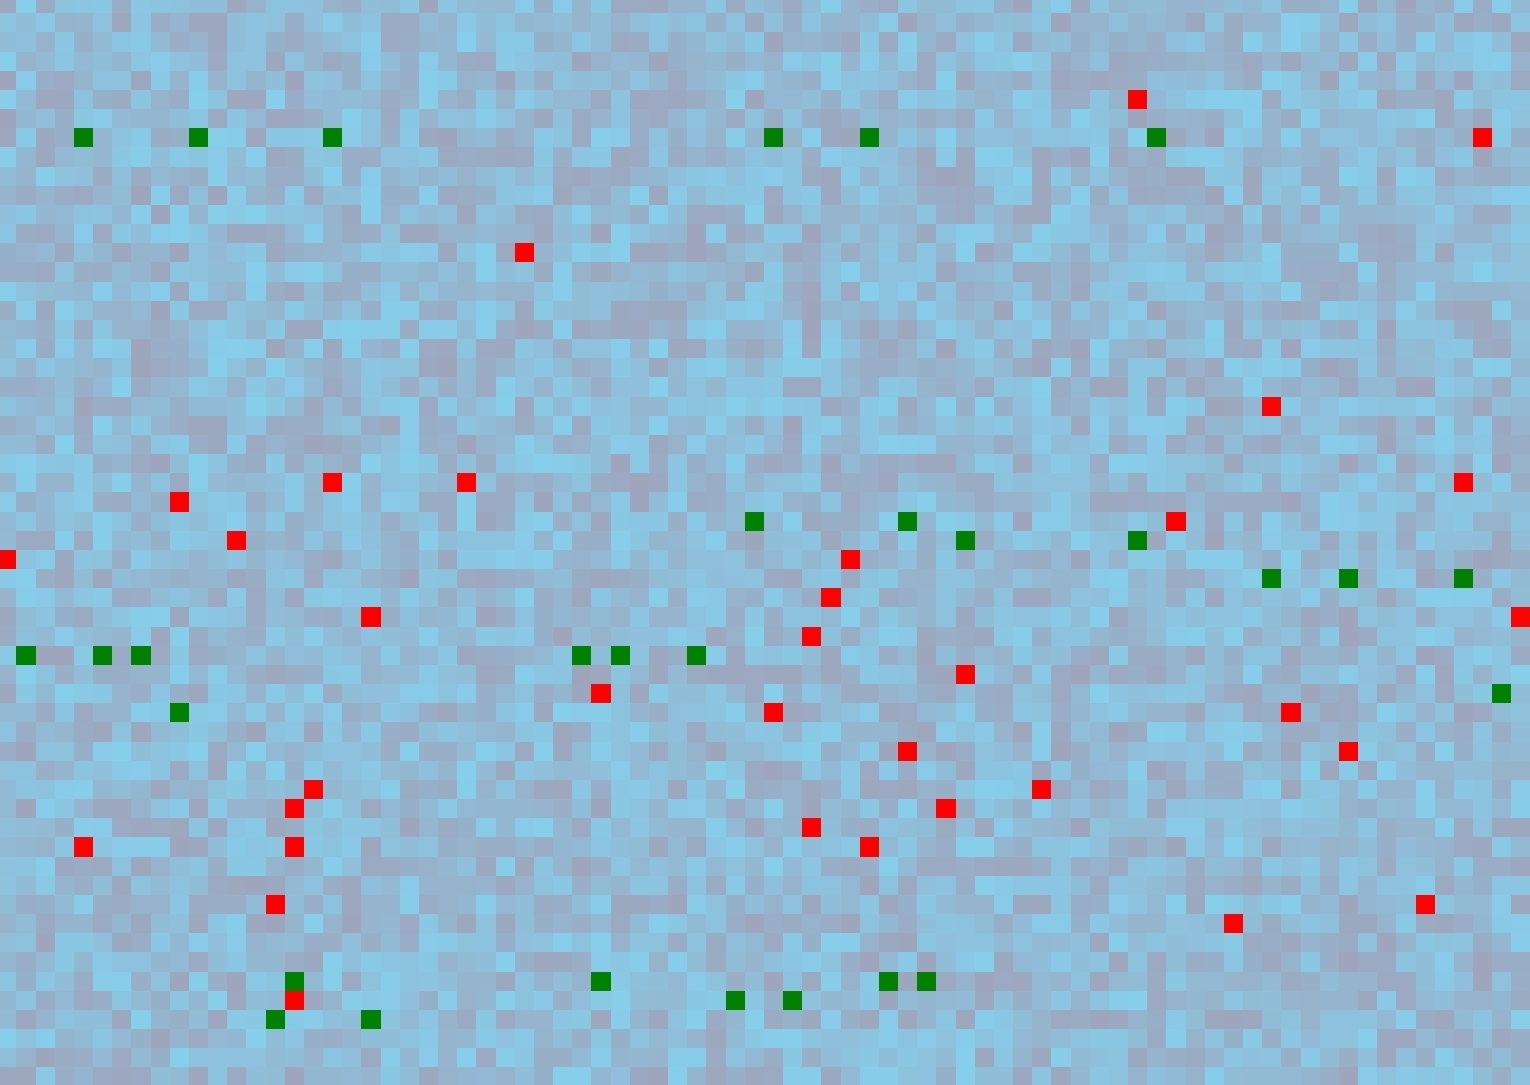
\includegraphics[width=\textwidth]{doc11358_topic0.jpg}
  \end{minipage}
  ~
  \begin{minipage}{0.20\textwidth}
    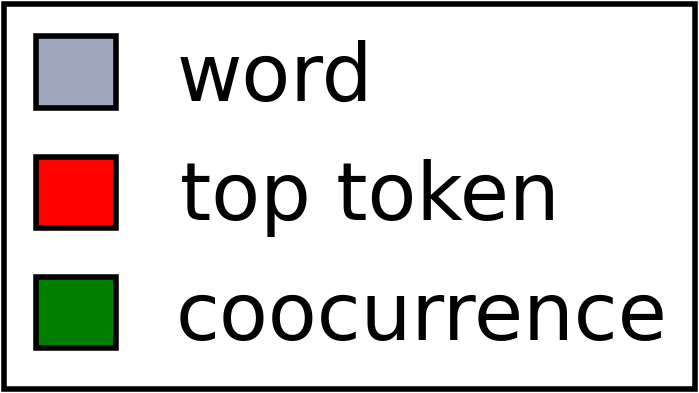
\includegraphics[width=\textwidth]{legend.png}
  \end{minipage}
  \begin{block}{Problem}
    Ten most frequent words cover only a small proportion of text.
    Сo-occurrences are even fewer.
    Can one rely on the analysis of these co-occurrences?
  \end{block}
\end{frame}

%\section{Цель исследования}
\begin{frame}{Purpose of the Study}
  \begin{block}{Problem}
    Top-tokens based coherences rely on the list of top ten words.\\
    These words reflect only a small part of the whole topic model.
  \end{block}
  \begin{block}{Solution}
    Evaluate coherence as an average thematic proximity of words closely located in text.
  \end{block}
\end{frame}


\iffalse
\begin{frame}
  \frametitle{Contents}
  \tableofcontents
\end{frame}
\fi


\section{Prologue}


\subsection{Topic Modeling}


\begin{frame}{Topic Modeling and Matrix Factorization}
  Topic model describes documents using \emph{latent} topics
  \smallskip
  
  \begin{itemize}
    \item $\phi_{wt} \equiv p(w \mid t)$~---~ how often word $w$ appears in topic $t$
    \item $\theta_{td} \equiv p(t \mid d)$~---~probability of topic $t$ within document $d$
  \end{itemize}
  
  \centering
  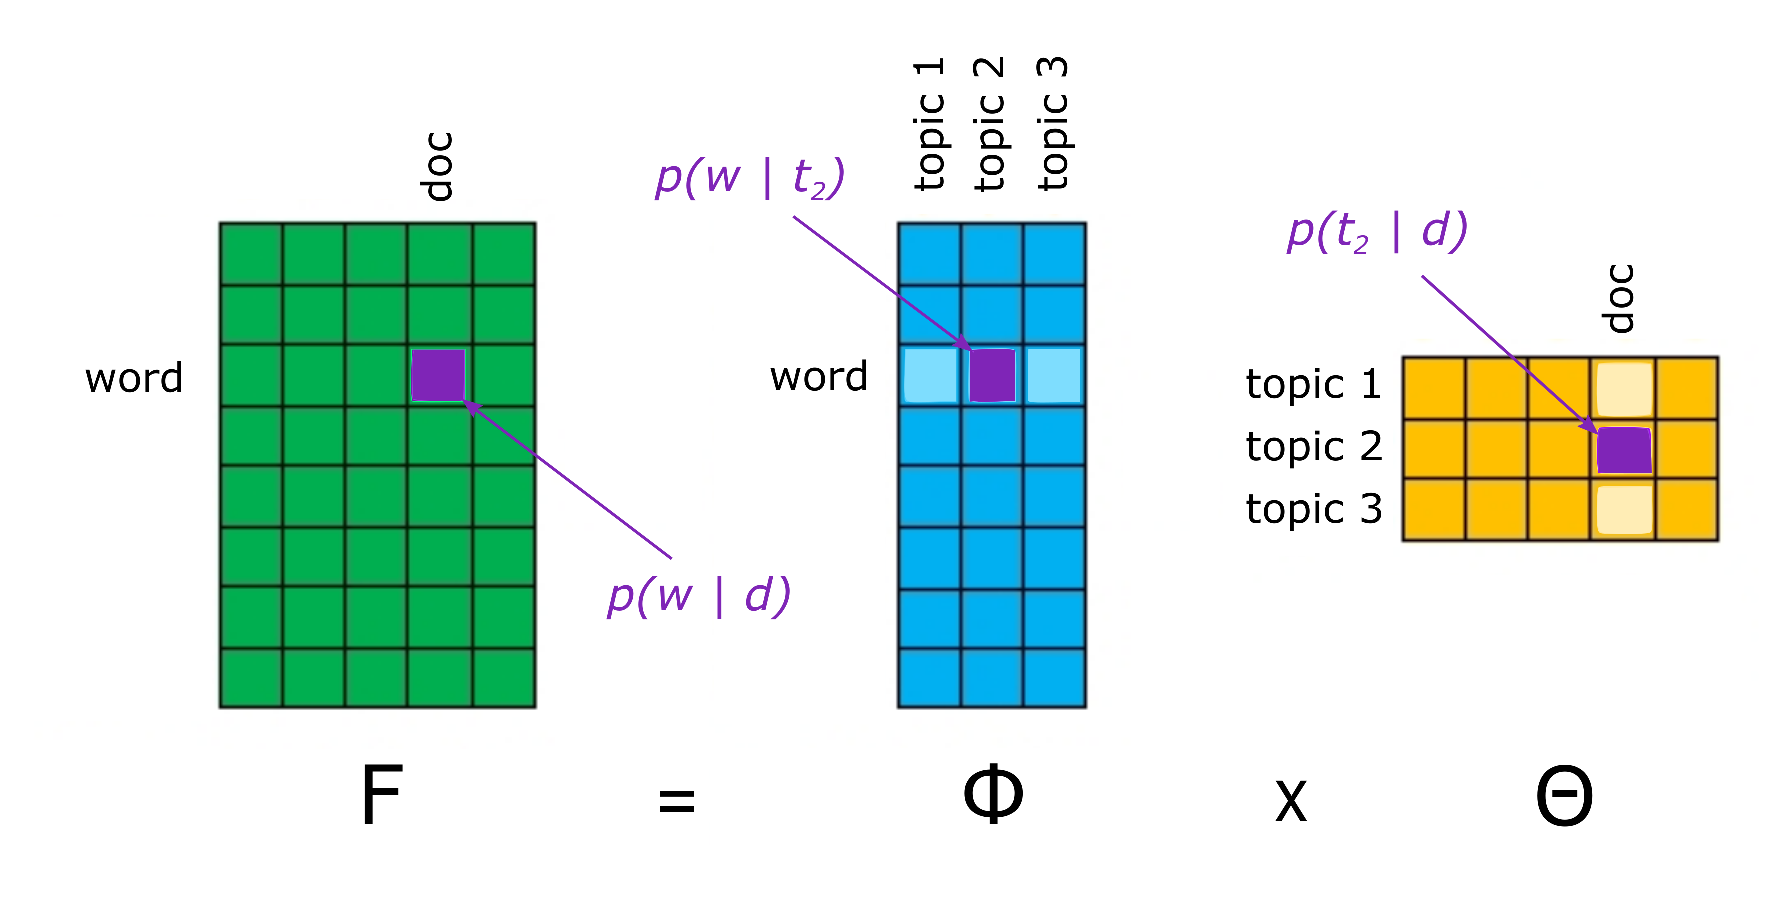
\includegraphics[width=\textwidth]{murat_plsa.eps}\\

\end{frame}

\subsection{Original Dataset}

\begin{frame}{Original Dataset: Three Top-Words of Each of 19 Topics}

  {\small
    $2000$ \emph{monotopic} PostNauka\footnote[frame]{https://postnauka.ru} articles. Topics found with BigARTM\footnote[frame]{Vorontsov K. et al. Bigartm: Open source library for regularized multimodal topic modeling of large collections, 2015}
  }
  
  \begin{figure}[h]
    \centering
    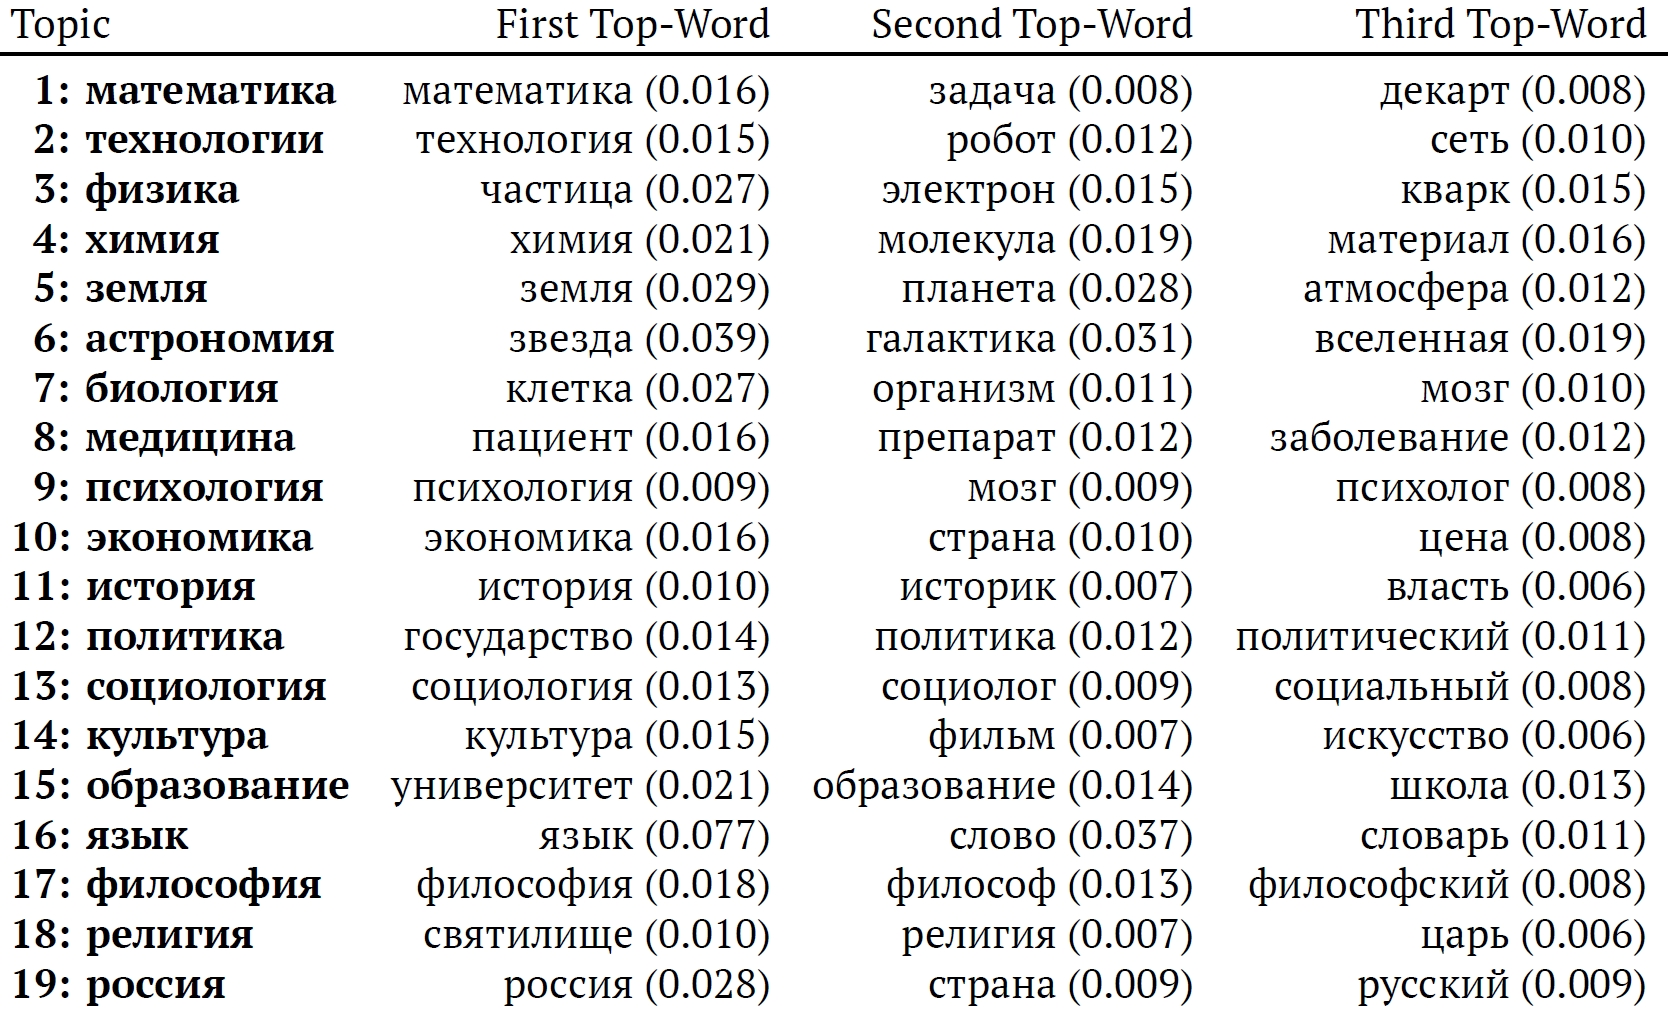
\includegraphics[width=0.85\textwidth]{topwords.jpg}
  \end{figure}
\end{frame}

\section{Top-Tokens Based Coherences}


\subsection{Newman, Mimno}

\begin{frame}{
  Newman, % ${}^{\mbox{\scriptsize 3}}$
  Mimno % ${}^{\mbox{\scriptsize 4}}$
}
  \begin{block}{}
  \begin{itemize}
    \setlength\itemsep{0.5cm}
    \item
      $
      \Newman\footnote[frame]{Newman et al. Automatic Evaluation of Topic Coherence, 2010}\Bigm|_{t}\, = \dfrac{1}{\binom{k}{2}} \sum\limits_{i=1}^{\textcolor{my-col1}{\bds k}-1}\sum\limits_{j=i+1}^{\textcolor{my-col1}{\bds k}} \ln \dfrac{p(w_i, w_j)}{p(w_i) p(w_j)}
      $
    \item
      $
      \Mimno\footnote[frame]{Mimno et al. Optimizing Semantic Coherence in Topic Models, 2011}\hphantom{n\,}\Bigm|_{t}\, = \dfrac{1}{\binom{k}{2}} \sum\limits_{i=1}^{\textcolor{my-col1}{\bds k}-1}\sum\limits_{j=i+1}^{\textcolor{my-col1}{\bds k}} \ln \dfrac{D(w_i, w_j) + 1}{D(w_i)}
      $
  \end{itemize}
  \end{block}
  
  \begin{itemize}
  \item $\textcolor{my-col1}{\bds k}$~---~number of top-words of topic $t$ used to evaluate coherence
  \item $p(w_i),\, p(w_i, w_j)$~---~probability to find word $w_i$ and two words $w_i, w_j$ in a context window of given size
  \item $D(w_i),\, D(w_i, w_j)$~---~number of documents containing word $w_i$ and two words $w_i, w_j$ in a context window of given size
  \end{itemize}
\end{frame}


\subsection{Drawbacks of Top-Tokens Based Approach}

\begin{frame}{Drawbacks of Top-Tokens Based Approach}
  Top token-based coherences may ignore more than 98\% of words of the documents' collection.
  
  \bigskip
  
  \begin{table}[h]
    \centering
    \captionsetup{justification=centering}
    
    \begin{tabular}{lcc}
      {} & PostNauka, \% & Wikipedia, \%\\
      \midrule
      Minimum & 0.016 & 0.0065\\
      Median & 0.048 & 0.029\\
      Mean & 0.062 & 0.036\\
      Maximum & 0.28 & 0.11\\
      \midrule
      Total & \textbf{1.2} & \textbf{1.7}
    \end{tabular}
    
    \caption*{The proportion of corpus contributing to the co-occurrence counts of top 10 most frequent words for each topic}
  \end{table}
\end{frame}


\begin{frame}{Drawbacks of Top-Tokens Based Approach}
  A single top token "частиц" out of the first 10 ones is seen.\\
  The wide range of less strong topical words is ignored by the top-tokens based coherences.
  \begin{figure}[h]
    \centering
    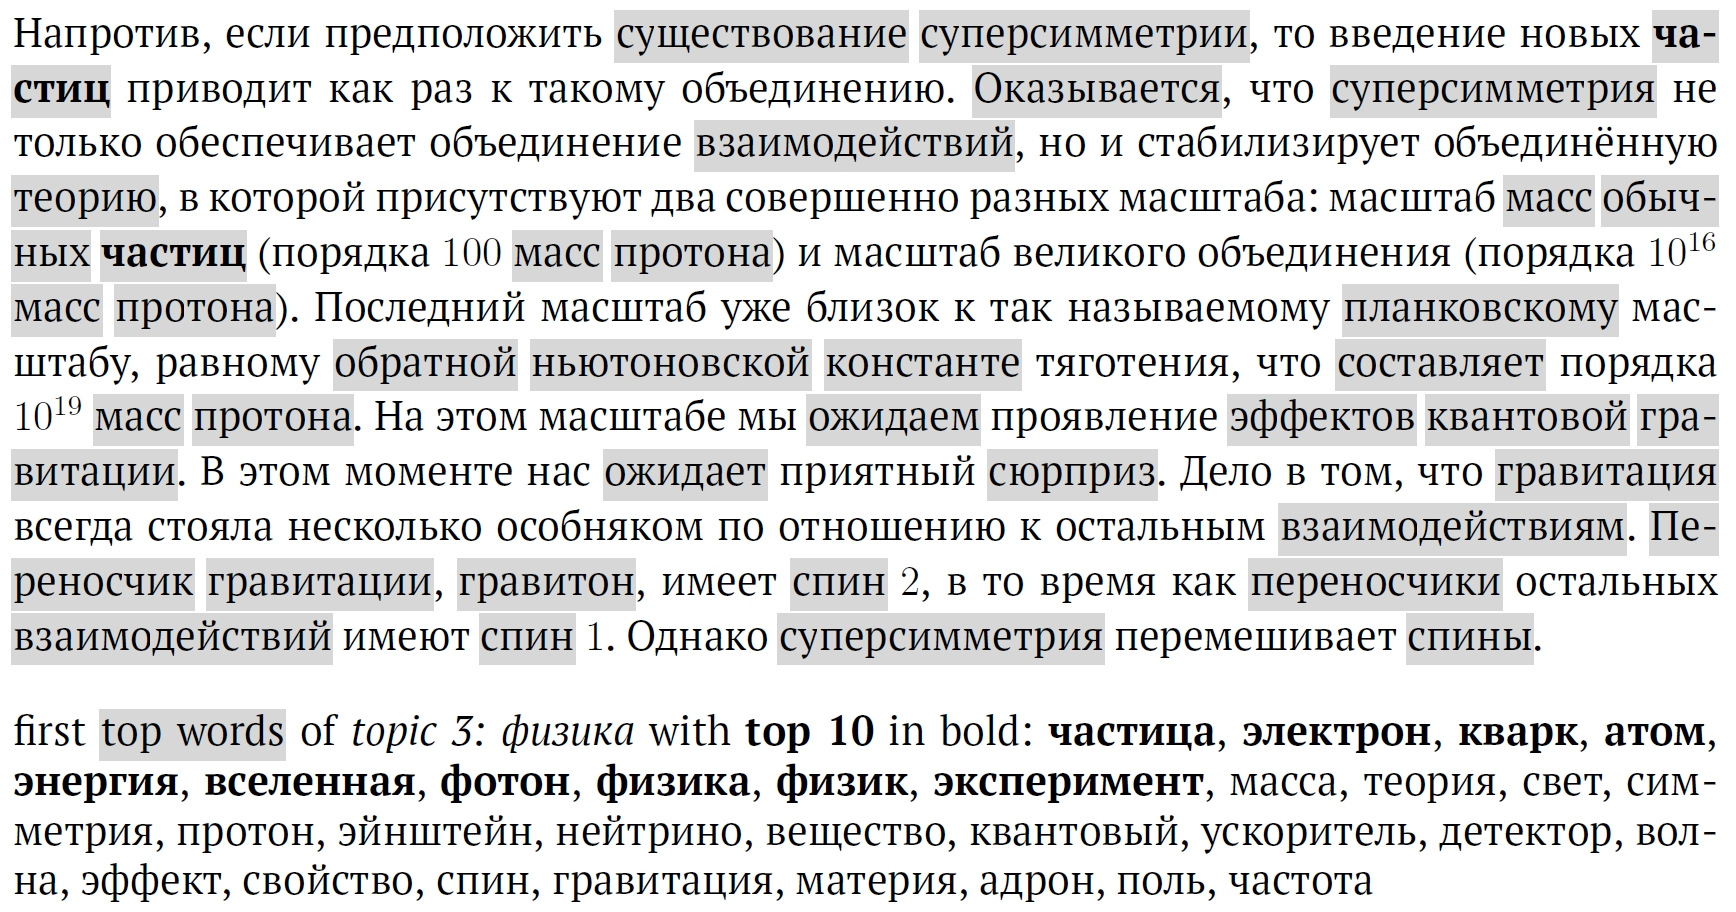
\includegraphics[width=1.0\textwidth]{topwords-insufficient.jpg}
  \end{figure}
\end{frame}


\section{Intra-Text Coherences}


\begin{frame}{SemantiC (L2, Cos)}

  \begin{block}{Meaning}
    Semantic proximity of closely located words in text
  \end{block}
\begin{table}[]
%\begin{tabular}{lllll}
\begin{tabularx}{320pt}{l| *{4}{Y}|}
%& Group of & astronomers & discovered & a star \\
& Группа & астрономов & обнаружила & звезду \\
\begin{tabular}[c]{@{}l@{}}$\begin{matrix}\\ \textcolor{my-red}{Astronomy} \\\\
\textcolor{my-green}{Biology} \\\\
\textcolor{blue}{Music} \\\\
\end{matrix}$\end{tabular} & 
\begin{tabular}[c]{@{}l@{}} 
    $\topicvector{my-red!10}{my-green!33}{blue!66}$
\end{tabular} & 
\begin{tabular}[c]{@{}l@{}}
    $\topicvector{my-red!90}{my-green!10}{blue!10}$
\end{tabular} &  
\begin{tabular}[c]{@{}l@{}}
    $\topicvector{my-red!45}{my-green!45}{blue!10}$
\end{tabular} & 
\begin{tabular}[c]{@{}l@{}}
    $\topicvector{my-red!75}{my-green!10}{blue!55}$
\end{tabular}
\end{tabularx}
\end{table}
Pairs of close vectors are compared: e.g. $\smalltopicvector{my-red!10}{my-green!33}{blue!66}$ vs $\smalltopicvector{my-red!75}{my-green!10}{blue!55}$
\end{frame}

\begin{frame}{SemantiC (Var)}

  \begin{block}{Meaning}
    How much the meanings of adjacent words differ, according to the topic model
  \end{block}
\begin{table}[]
\small
\begin{tabularx}{1.0\textwidth}{l| *{3}{Y}|*{3}{Y}|}
& \multicolumn{3}{c|}{Low variance} 
& \multicolumn{3}{c|}{High variance}\\
\cline{2-7}
& русский & поэт & Пушкин & Толстой & Рассел & Эйлер \\
\begin{tabular}[c]{@{}l@{}}$\begin{smallmatrix}\\ \textcolor{my-red}{Literature} \\\\
\textcolor{my-green}{Philosophy} \\\\
\textcolor{blue}{Mathematics} \\\\
\end{smallmatrix}$\end{tabular}  &
\begin{tabular}[c]{@{}l@{}} 
    $\smalltopicvector{my-red!50}{my-green!25}{blue!25}$
\end{tabular} & 
\begin{tabular}[c]{@{}l@{}}
    $\smalltopicvector{my-red!90}{my-green!10}{blue!10}$
\end{tabular} &  
\begin{tabular}[c]{@{}l@{}}
    $\smalltopicvector{my-red!90}{my-green!10}{blue!10}$
\end{tabular} &  
\begin{tabular}[c]{@{}l@{}}
    $\smalltopicvector{my-red!90}{my-green!30}{blue!10}$
\end{tabular} &  
\begin{tabular}[c]{@{}l@{}}
    $\smalltopicvector{my-red!10}{my-green!50}{blue!50}$
\end{tabular} &  
\begin{tabular}[c]{@{}l@{}}
    $\smalltopicvector{my-red!10}{my-green!10}{blue!90}$
\end{tabular}  
\end{tabularx}
\end{table}
\end{frame}


\begin{frame}{TopLen}
  \begin{block}{Meaning}
    Average length of the topic in text
  \end{block}
  
  \medskip
  
  Count words of topic $t$, penalizing when word of another topic is encountered.
  
  \medskip
  
  \begin{exampleblock}{Пример. Тема $t = \mbox{"Чёрные дыры"}$}
  \noi
  $\mbox{Группе}\ \underbrace{\mbox{\textcolor{my-pink}{астрономов}}\ \mbox{удалось}}_{l_1=2}\ \mbox{обнаружить}\ \underbrace{\mbox{\textcolor{my-pink}{звезду}}, \mbox{обращающуюся}}_{l_2=2}$\\
  $\mbox{вокруг}\ \underbrace{\mbox{\textcolor{my-red}{чёрной}}\ \mbox{\textcolor{my-red}{дыры}}\ \mbox{на}\ \mbox{рекордно}\ \mbox{близком}}_{l_3=4}\ \mbox{расстоянии}.$
  \end{exampleblock}
\end{frame}


\begin{frame}{FoCon}
  \begin{block}{Meaning}
    Estimation of how much the focus of a conversation drifts
  \end{block}
  
  \begin{figure}[h]
    \centering
    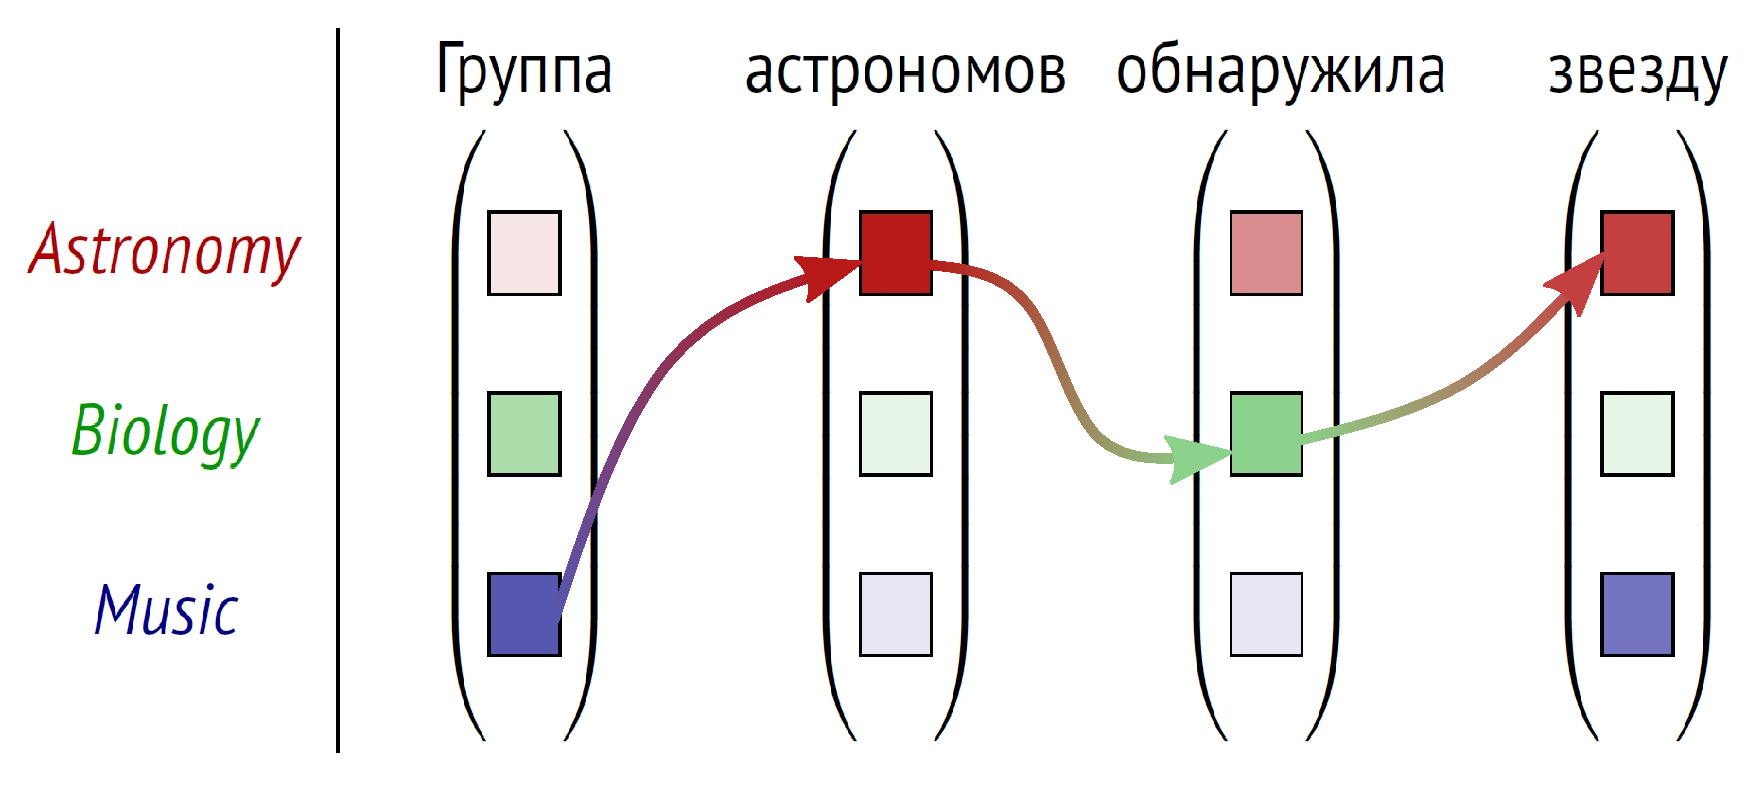
\includegraphics[width=1.0\textwidth, height=0.45\textheight]{astronomers_focon.eps} % .eps image is wrong scaled
  \end{figure}
\end{frame}


\section{Automatic Coherences' Quality Estimation}


\subsection{Semisynthetic Dataset}
\begin{frame}
  \frametitle{Motivation}
  \begin{block}{}
    The better the coherence is, the better it should describe the ability of a topic model to figure out the segmentation structure!
  \end{block}   
  \begin{figure}[h]
    \centering
    \includegraphics[width=0.7\textwidth, height=0.5\textheight]{pn_gen_diagram.eps}
    \caption*{Document consisting of sociology and medicine segments}
  \end{figure}    
\end{frame}


\begin{frame}{Dataset Generation}
  \begin{columns}
  \column{0.5\textwidth}
    \begin{itemize}\setlength{\itemindent}{-1em} % https://stackoverflow.com/questions/2611276/latex-beamer-way-to-change-the-bullet-indentation
      \item We “cut” the monotopical documents into smaller monotopical segments.
      \item We “sew” them together in random order to produce a new document. 
      \item We know topic labels for each word and can use them as ground truth.
    \end{itemize}
    
  \column{0.5\textwidth}
  
    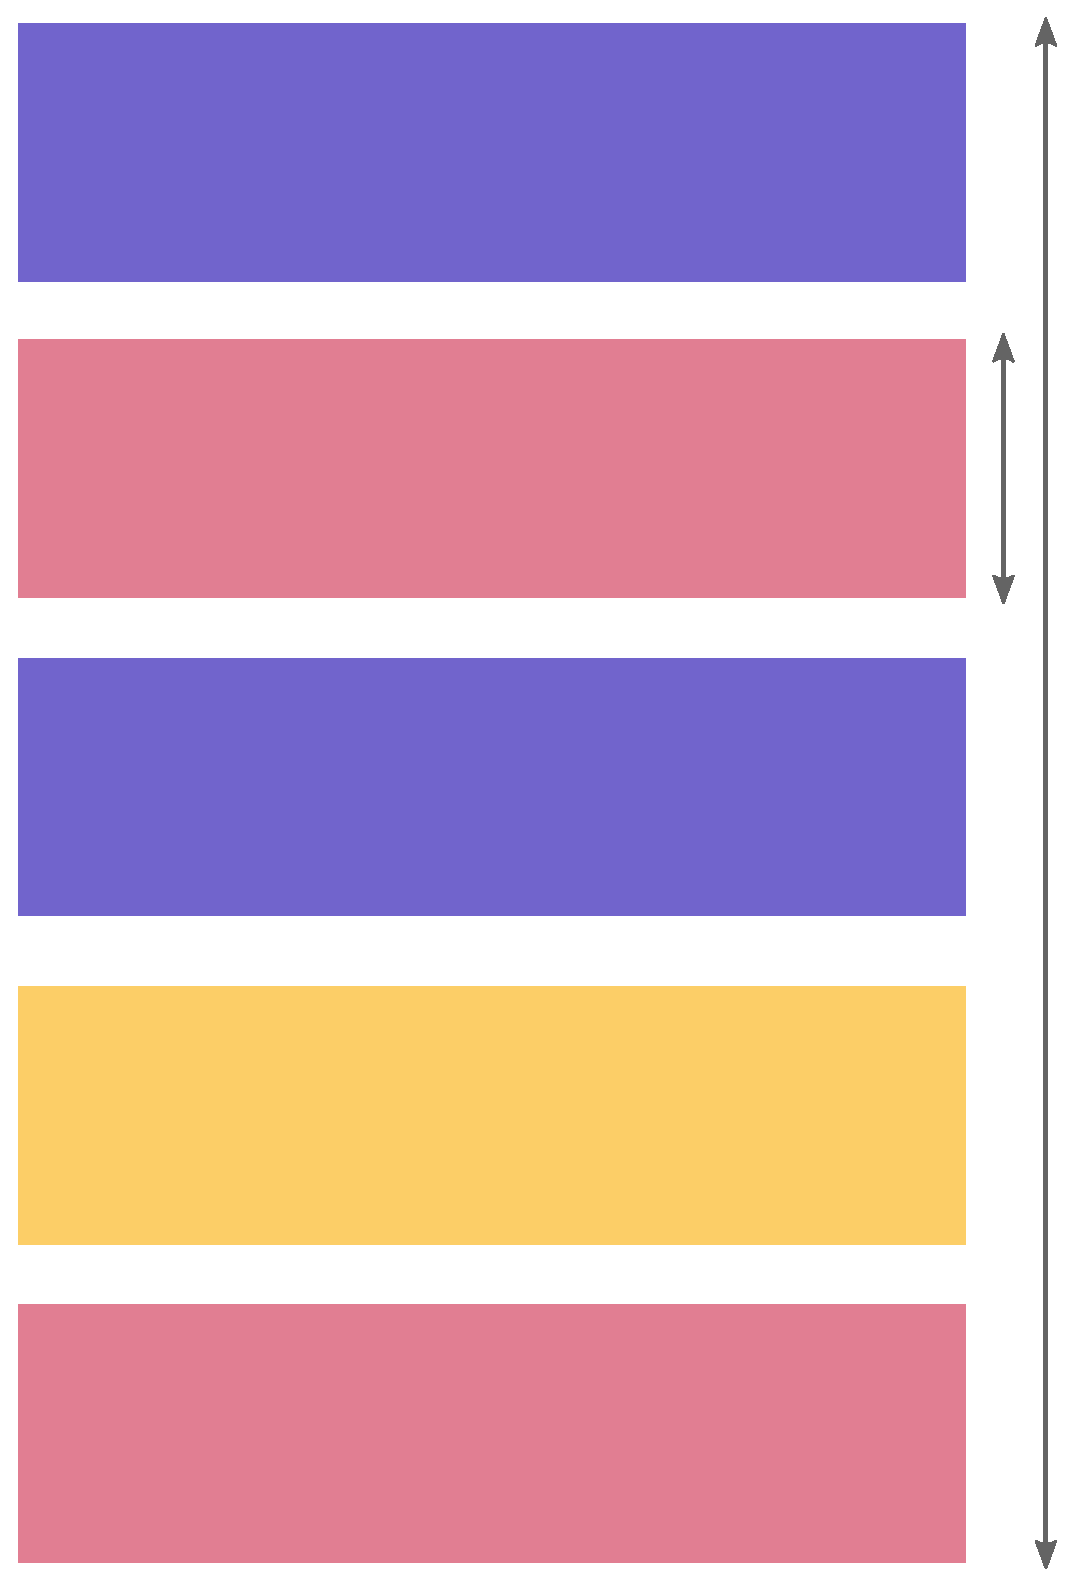
\includegraphics[width=0.95\linewidth, height=0.6\textheight]{dataset} % scale=0.20
  \end{columns}
  
  \medskip
  
\end{frame}

	
\subsection{Segmentation Quality}


\begin{frame}{Segmentation Quality}
  \begin{block}{Soft}
    Sum among topics of sums $p(t \mid d, w)$ for each topic $t$ over pairs $(d, w), d \hm\in d, w \hm\in W_d$
  \end{block}
  
  \begin{block}{Strict}
    Number of coincidences of the topic $\argmax_\tau p(\tau \mid d, w)$ predicted by the model for the word $w$ in the document with the actual topic $t$ of the segment
  \end{block}
\end{frame}


\section{Experiments}


\begin{frame}{Illustration of \textbf{a Bad Model} Segmenting Text}
  \begin{figure}[h]
    \centering
    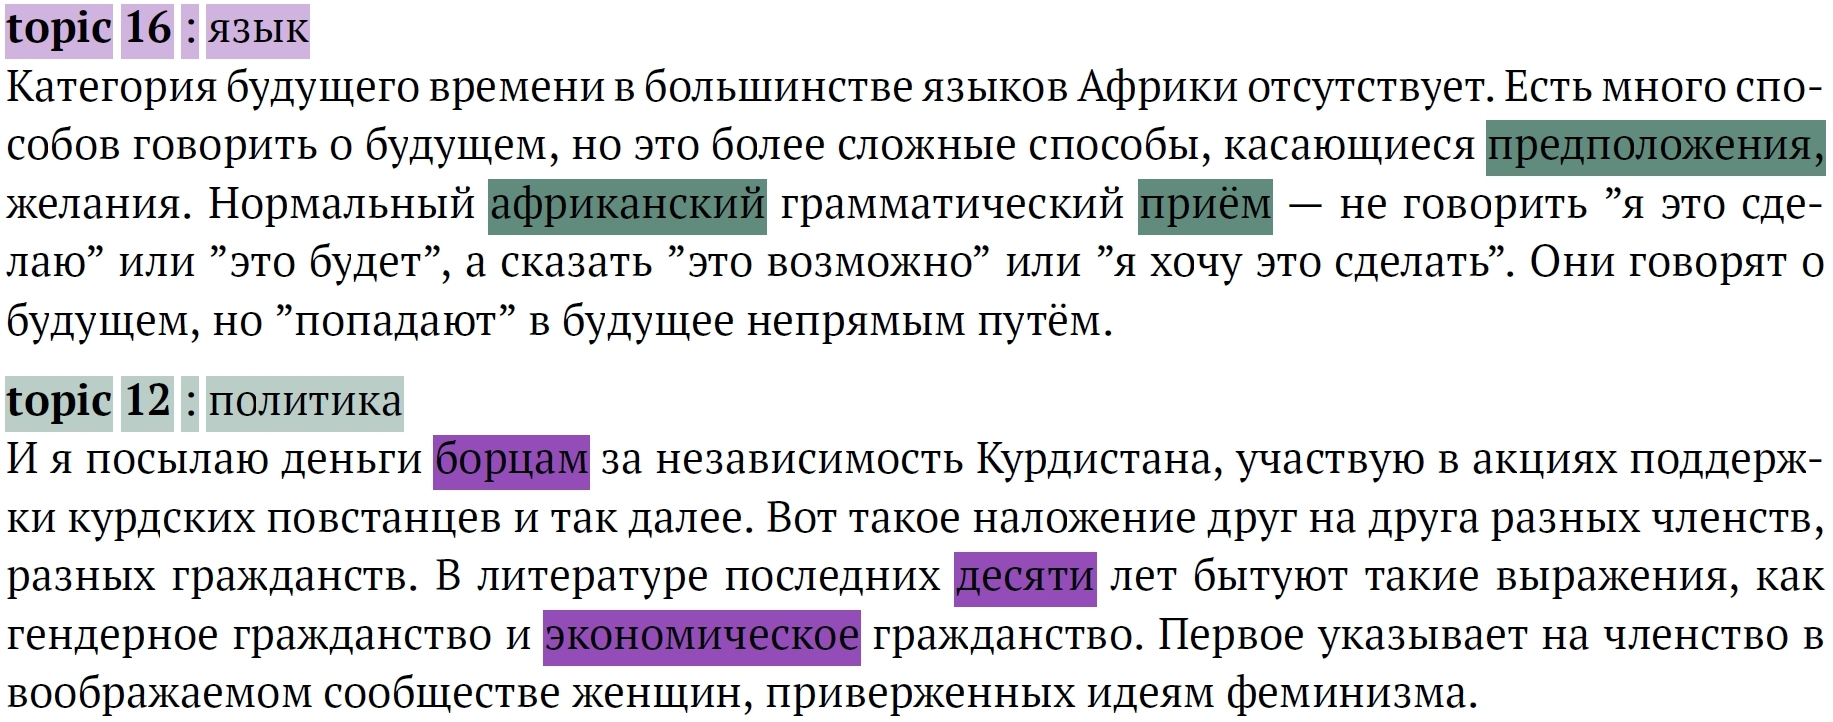
\includegraphics[width=\textwidth]{combine_bad.jpg}
  \end{figure}
  
  \vspace{-0.5cm}

  \begin{table}[h]
    \scriptsize
    \centering
    \begin{tabular}{rrrrrrrrr}
      SQ (S) & SQ (H) & N & M & SC L2 & SC Cos & SC Var & TL & FC\\
      \midrule
      \rowcolor{my-blue-light}
      5.54e3 & 1.10e4 & -4.83 & -3.12 & -12.9 & 0.947 & -37.0e3 & 2.87 & -13.9e4\\
      \textbf{16.0e3} & \textbf{3.76e4} & \textbf{-3.65} & \textbf{-2.69} & \textbf{-3.70} & 0.700 & \textbf{-8.12e3} & \textbf{3.45} & \textbf{-5.44e4}
    \end{tabular}
  \end{table}
  
  \begin{itemize}\setlength{\itemindent}{0pt}
    \small
    \item SQ (S), SQ (H)~---~Soft and Strict segmentation qualities
    \item N, M~---~Newman, Mimno
    \item SC, TL, FC~---~SemantiC, TopLen, FoCon
  \end{itemize}
\end{frame}


\begin{frame}{Illustration of \textbf{the Good Model} Segmenting Text}
  \begin{figure}[h]
    \centering
    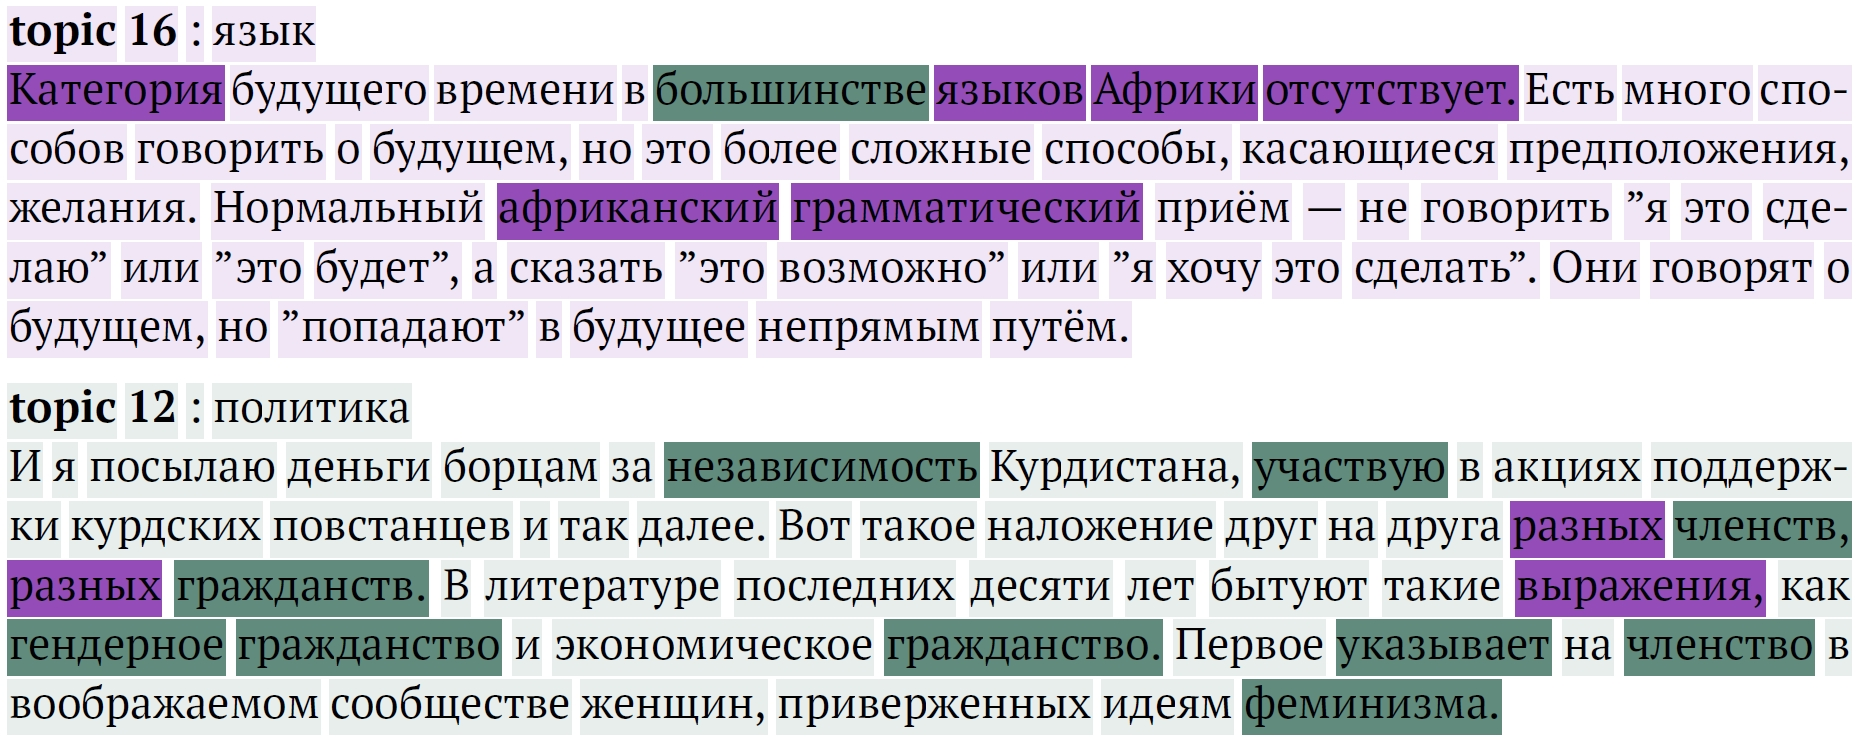
\includegraphics[width=\textwidth]{combine_good.jpg}
  \end{figure}
    
  \vspace{-0.5cm}

  \begin{table}[h]
    \scriptsize
    \centering
    \begin{tabular}{rrrrrrrrr}
      SQ (S) & SQ (H) & N & M & SC L2 & SC Cos & SC Var & TL & FC\\
      \midrule
      5.54e3 & 1.10e4 & -4.83 & -3.12 & -12.9 & 0.947 & -37.0e3 & 2.87 & -13.9e4\\
      \rowcolor{my-blue-light}
      \textbf{16.0e3} & \textbf{3.76e4} & \textbf{-3.65} & \textbf{-2.69} & \textbf{-3.70} & 0.700 & \textbf{-8.12e3} & \textbf{3.45} & \textbf{-5.44e4}
    \end{tabular}
  \end{table}
  
  \begin{itemize}\setlength{\itemindent}{0pt}
    \small
    \item SQ (S), SQ (H)~---~Soft and Strict segmentation qualities
    \item N, M~---~Newman, Mimno
    \item SC, TL, FC~---~SemantiC, TopLen, FoCon
  \end{itemize}
\end{frame}


\iffalse
\begin{frame}{Segmentation Quality \& Perplexity of Topic Model}
  \begin{itemize}\setlength{\itemindent}{-1em}
  \item Perplexity: intrinsic quality criteria; the lower, the better.
  \item Range of topic models: $\Phi(\alpha) = \alpha \Phi_{bad} + (1 - \alpha) \Phi_{good}$.
  \end{itemize}
  
  \begin{figure}[h]
    \centering
    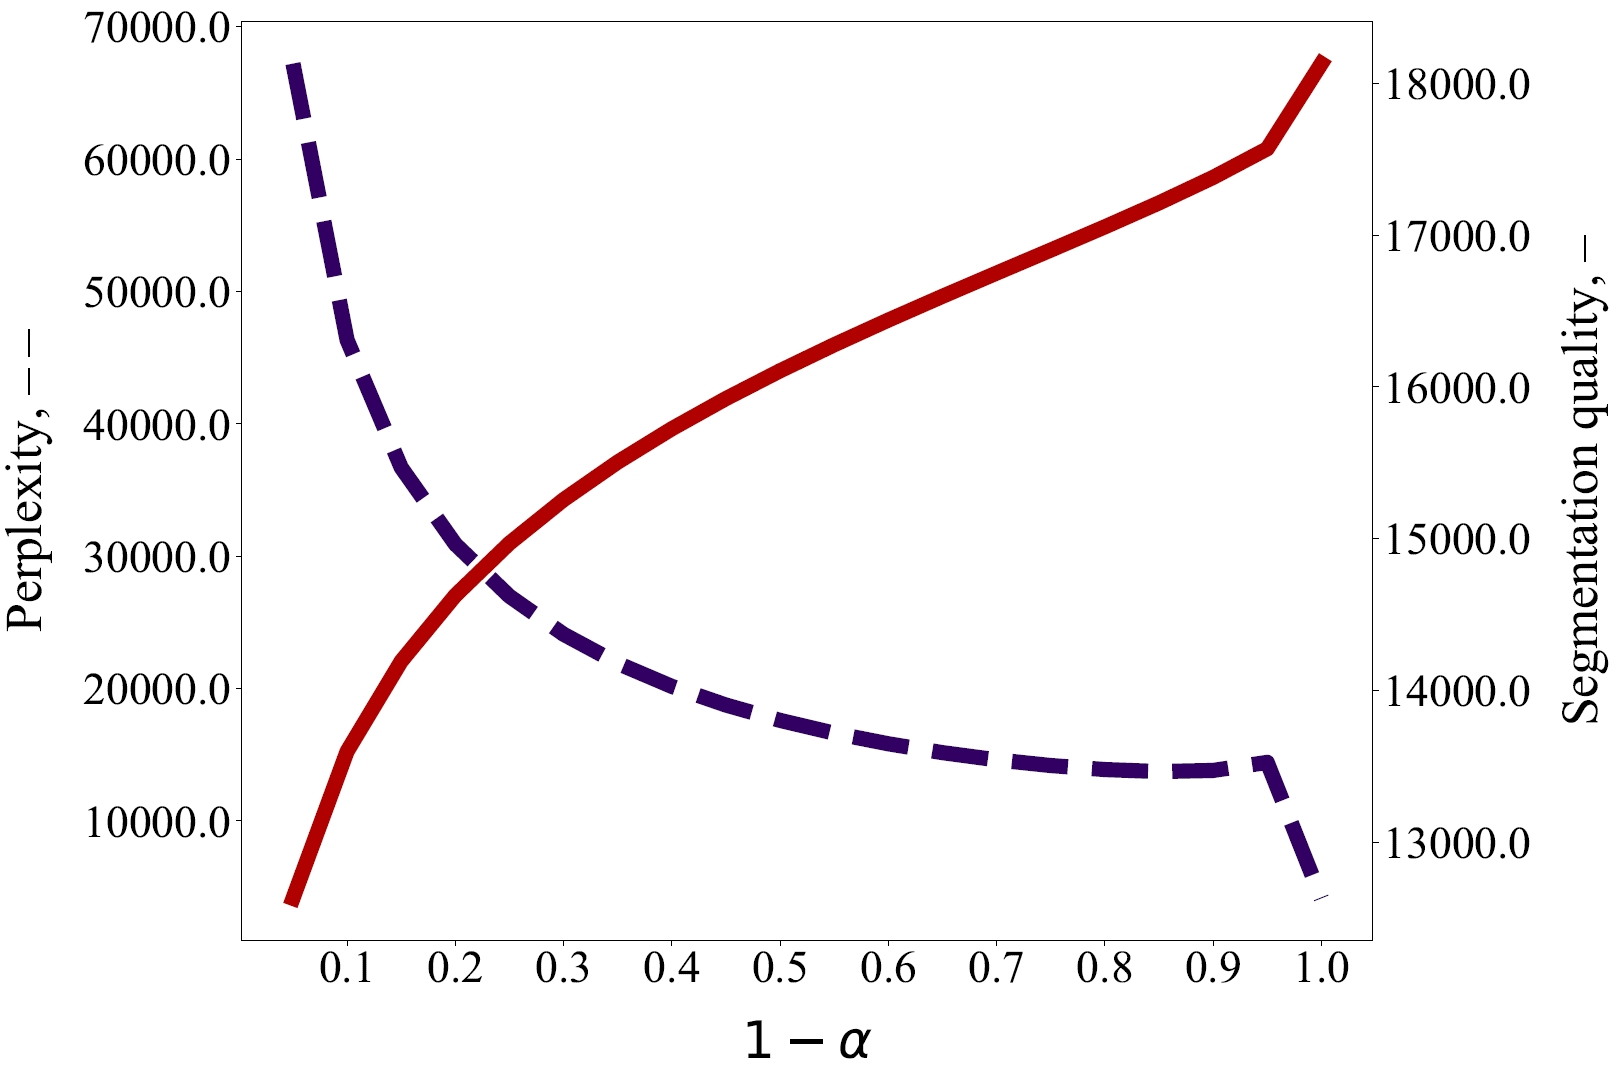
\includegraphics[width=0.65\textwidth]{segm_quality-iteration200}
  \end{figure}
  
  \begin{block}{}
    Proposed segmentation quality estimation may be used as topic models’ quality measure
  \end{block}
\end{frame}
\fi


\begin{frame}{Spearman Correlations Between\\Coherences \& Segmentation Quality}
  \begin{table}[t]
    \begin{tabular}{lr}
      Coh & Corr\\
      \toprule
      Newman & $0.75$\\
      Mimno & $0.96$\\
      \midrule
      SC L2 & $0.92$\\
      SC Cos & $-0.97$\\
      SC Var & $\mathbf{1.00}$\\
      TopLen & $\mathbf{1.00}$\\
      FoCon & $\mathbf{1.00}$\\
      \bottomrule
    \end{tabular}
    ~
    \begin{tabular}{lr}
      Coh & Corr\\
      \toprule
      Newman & $0.80$\\
      Mimno & $0.94$\\
      \midrule
      SC L2 & $0.70$\\
      SC Cos & $-0.97$\\
      SC Var & $\mathbf{1.00}$\\
      TopLen & $\mathbf{1.00}$\\
      FoCon & $\mathbf{1.00}$\\
      \bottomrule
    \end{tabular}
    ~
    \begin{tabular}{lr}
      Coh & Corr\\
      \toprule
      Newman & $0.85$\\
      Mimno & $0.97$\\
      \midrule
      SC L2 & $0.59$\\
      SC Cos & $-0.96$\\
      SC Var & $\mathbf{1.00}$\\
      TopLen & $\mathbf{1.00}$\\
      FoCon & $\mathbf{1.00}$\\
      \bottomrule
    \end{tabular}
    \centering
    \captionsetup{justification=centering}
    \caption*{
      Results for datasets with sizes of segments: 50, 200 and 400 words~---~and with $5$ topics in each document}
  \end{table}
\end{frame}


\begin{frame}{Coherences \& Segmentation Quality\\as Functions of Topic Model Quality}
  % dataset $\sgm=200,\ \thm=5$
  
  \begin{figure}[h]
    \begin{subfigure}[t]{0.48\textwidth}
      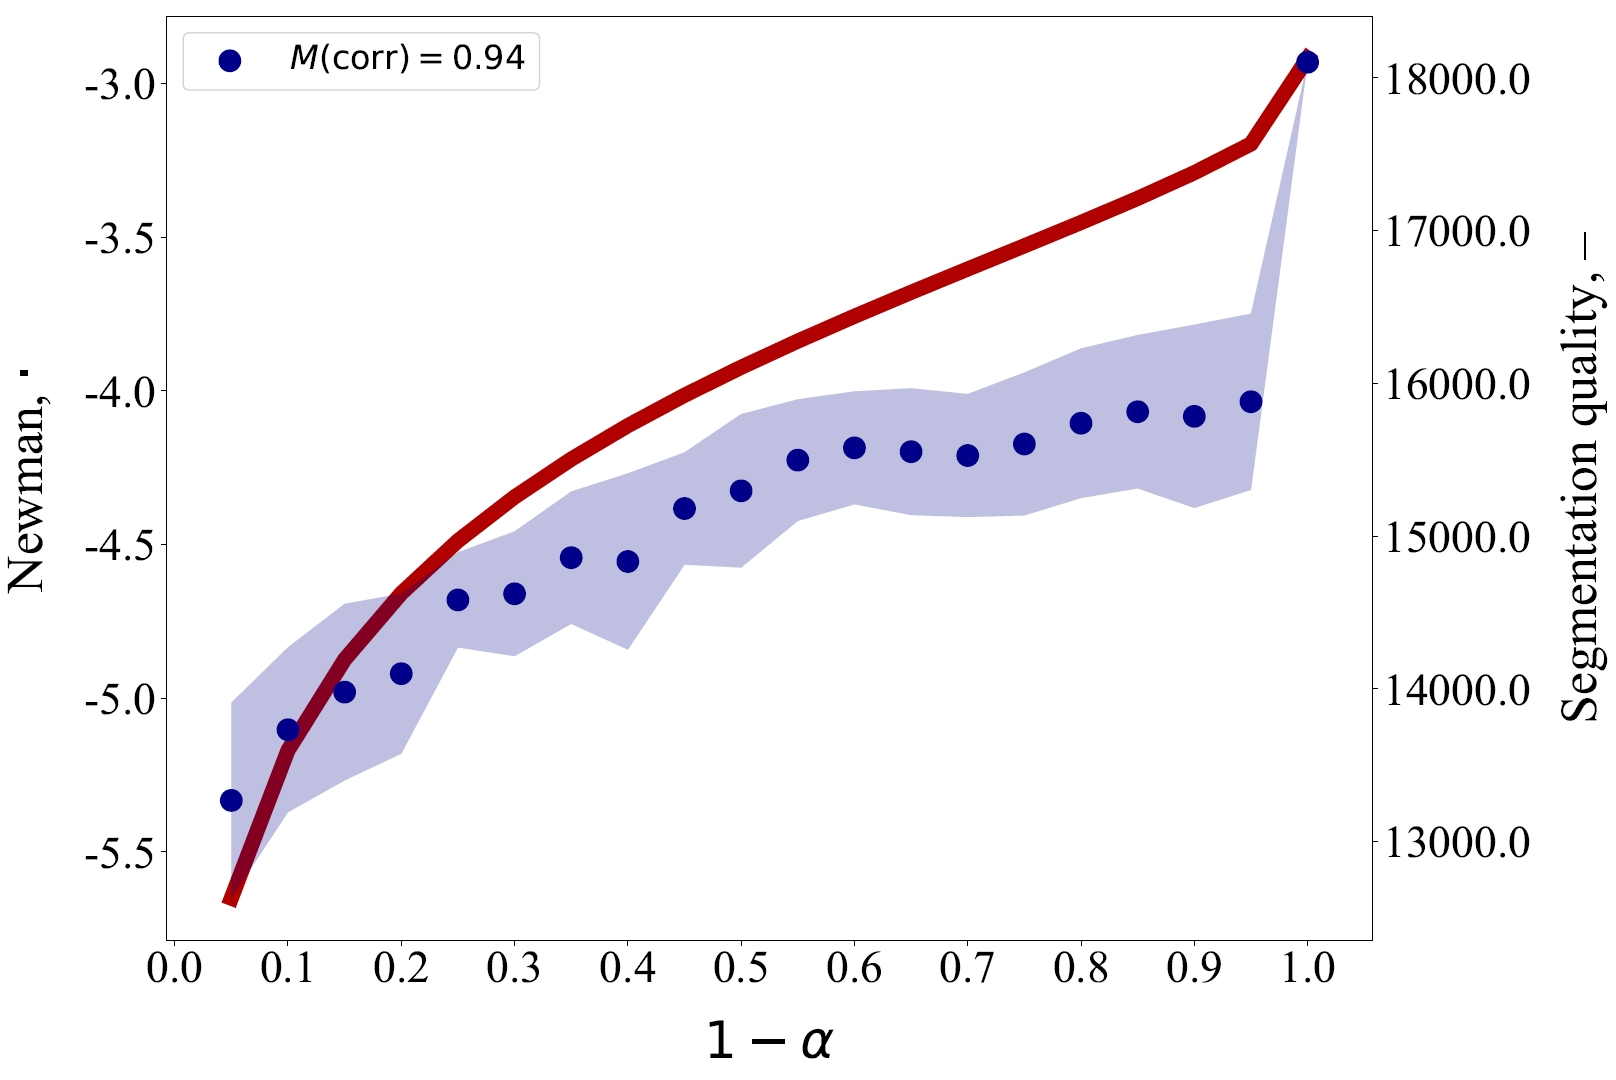
\includegraphics[width=\linewidth]{newman-iteration.jpg}
    \end{subfigure}
    ~
    \begin{subfigure}[t]{0.48\textwidth}
      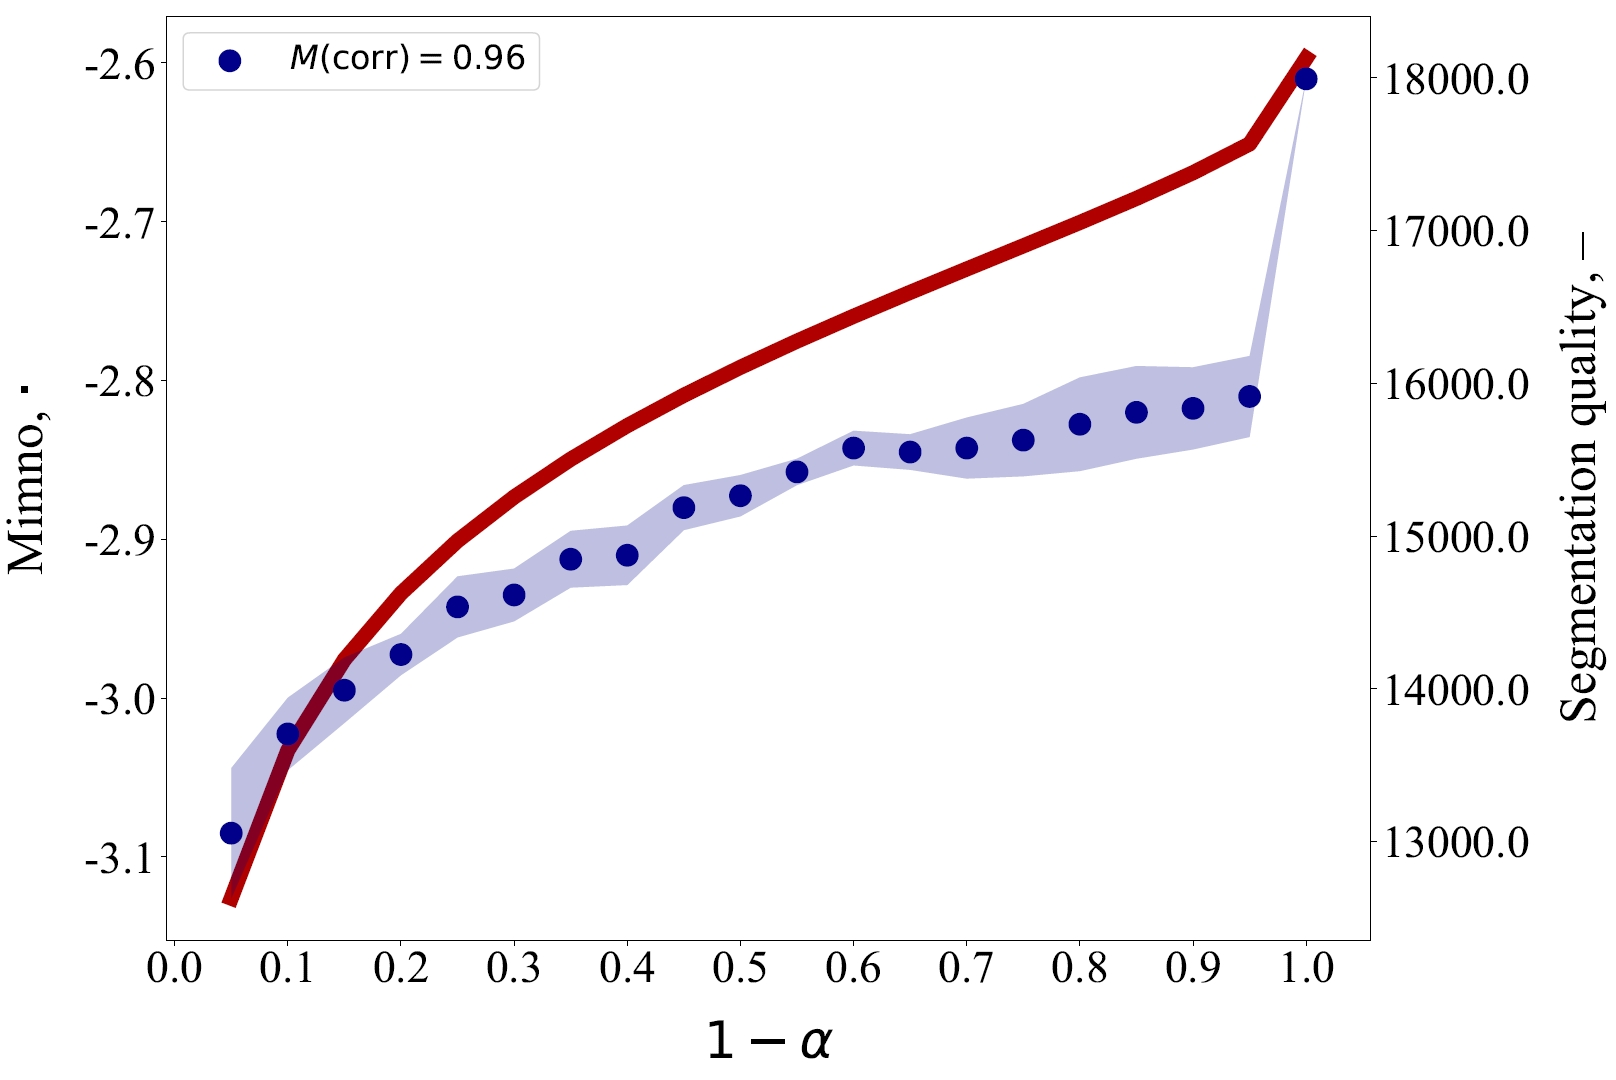
\includegraphics[width=\linewidth]{mimno-iteration.jpg}
    \end{subfigure}
    %%
    \begin{subfigure}[t]{0.48\textwidth}
      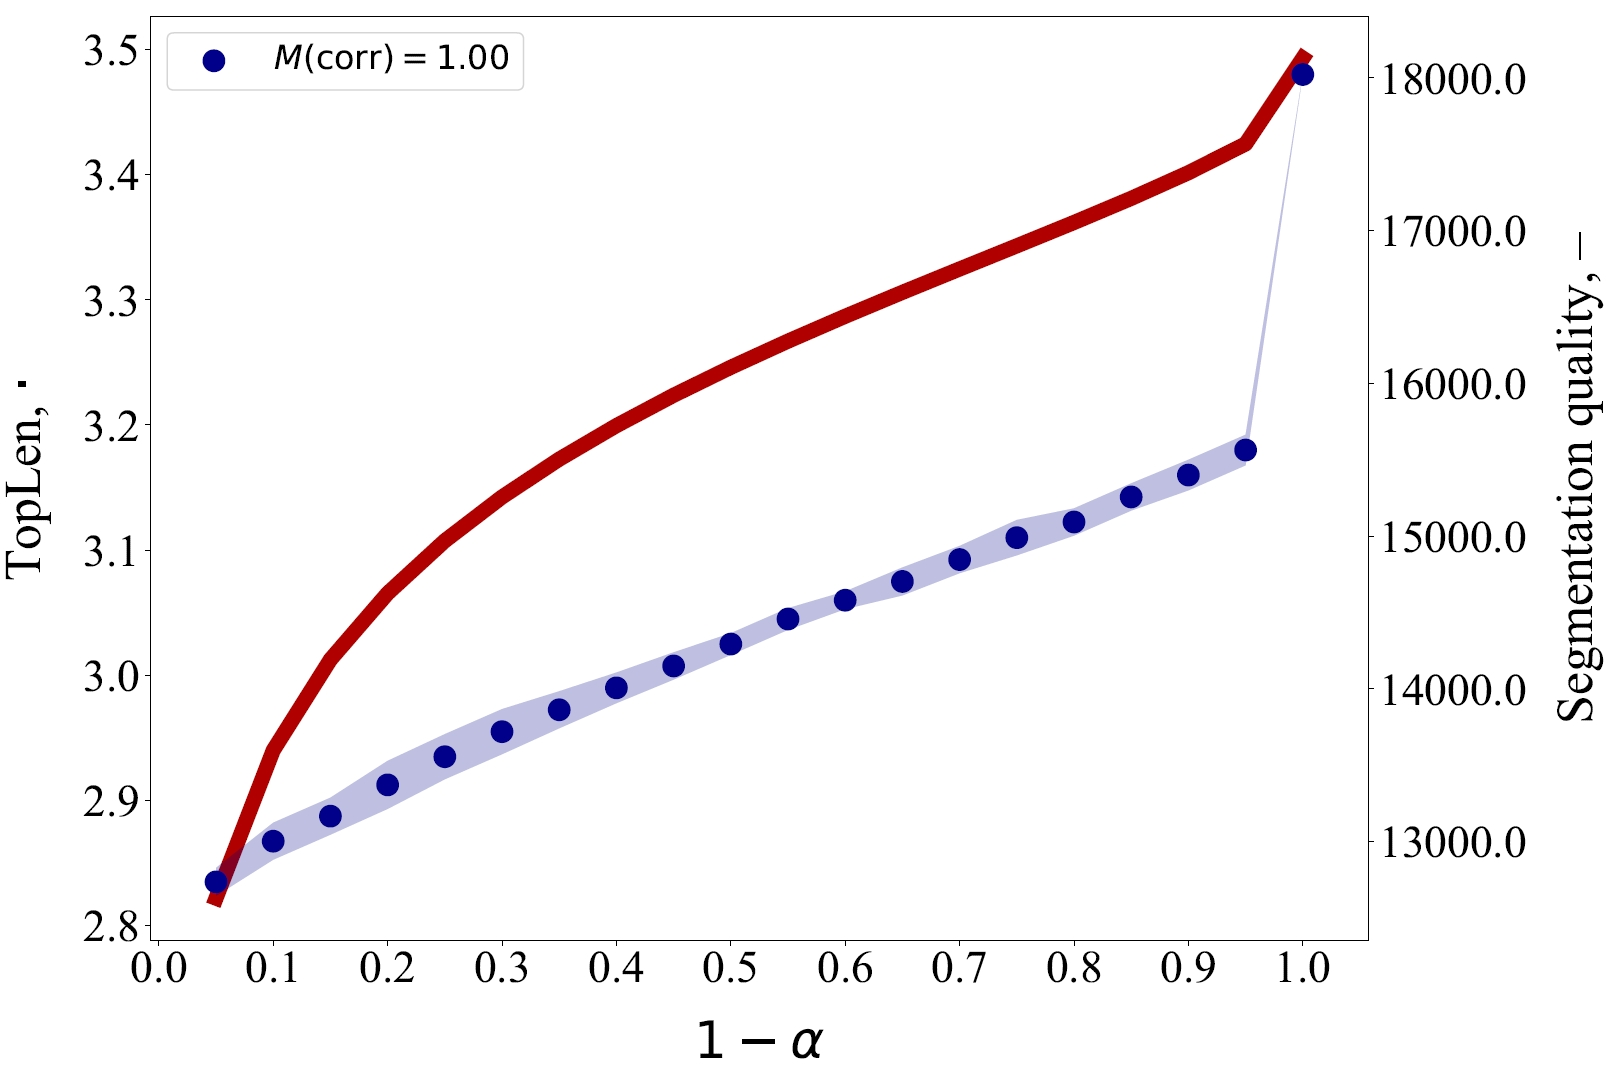
\includegraphics[width=\linewidth]{toplen-iteration.jpg}
    \end{subfigure}
    ~
    \begin{subfigure}[t]{0.48\textwidth}
      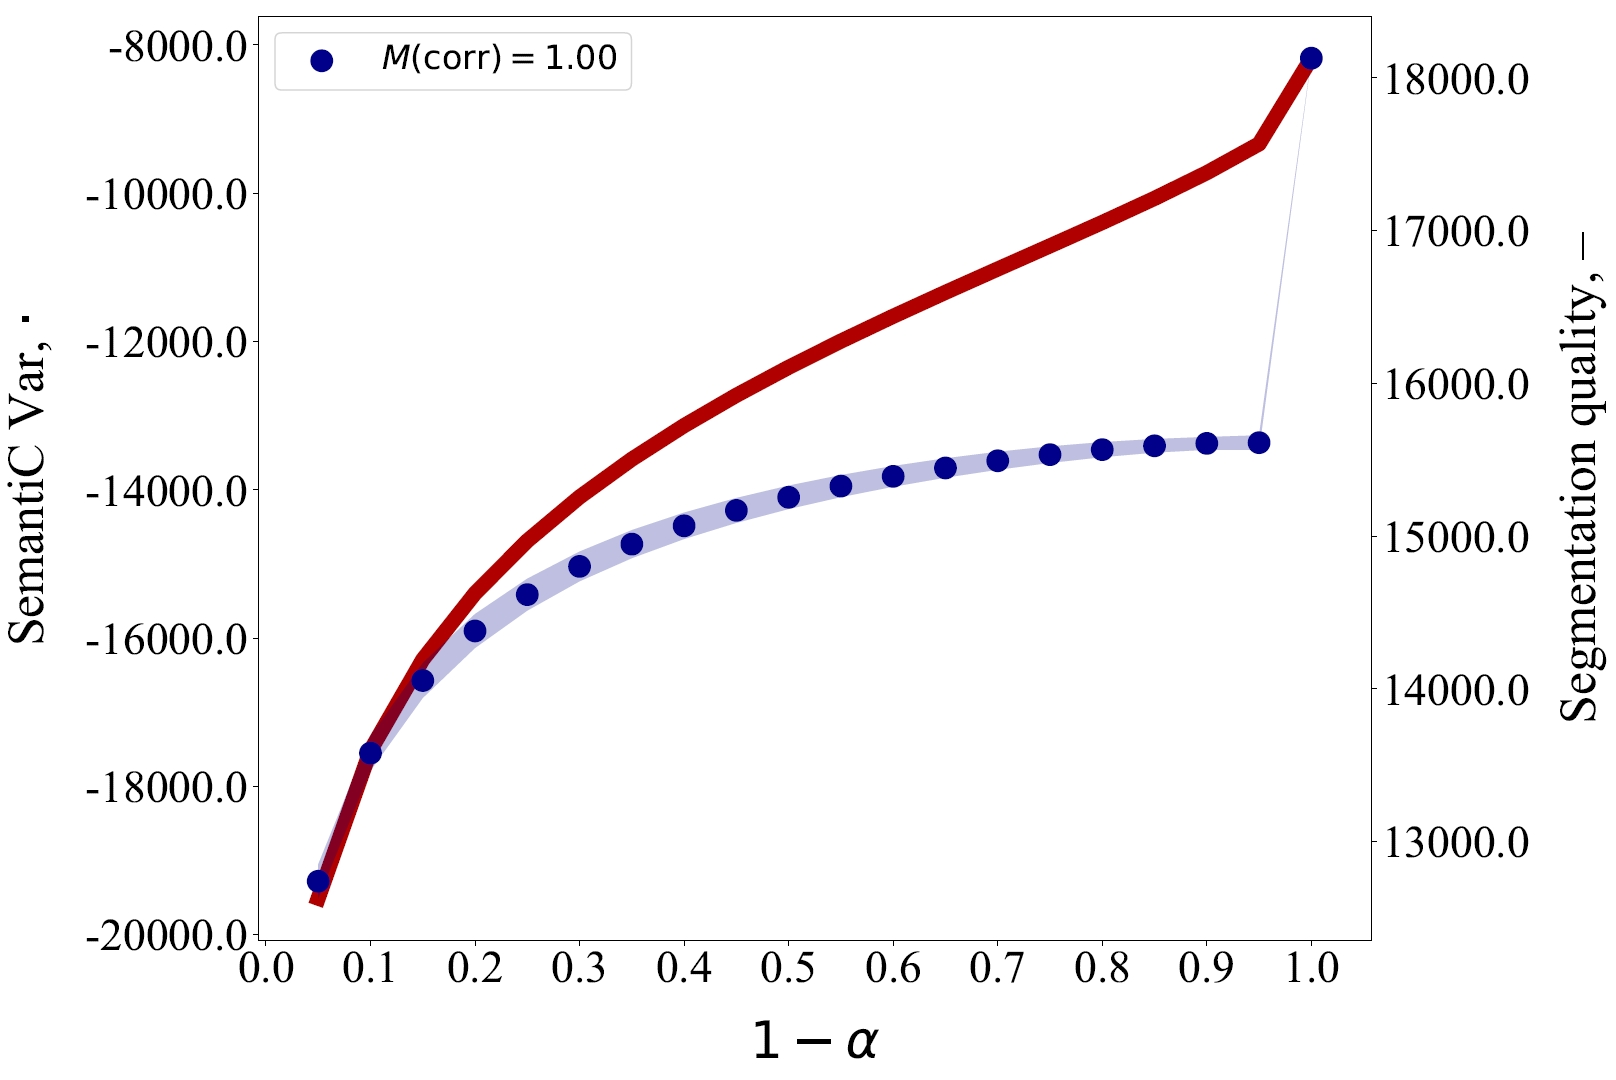
\includegraphics[width=\linewidth]{semantic_var-iteration.jpg}
    \end{subfigure}
  \end{figure}
\end{frame}

\begin{frame}{Results}
  \begin{itemize}
  \setlength\itemsep{0.5cm}
  \item
    New methods of calculating coherence of a topic are proposed.
    
    \smallskip
    
    These methods take into account the whole text and, in the problem under consideration, outperform the top-tokens based ones.
  \item
    An automatic method for evaluating coherences functions is introduced.
    
    \smallskip
    
    It is based on the comparison of coherence values with text segmentation qualities for a range of topic models.
  \end{itemize}
\end{frame}
\end{document}